\documentclass[10pt]{article}
% Packages
\usepackage{makecell} % For thicker lines
\usepackage{setspace}  % Controls line spacing
\usepackage{hhline}   % For double horizontal lines
\usepackage{colortbl}  % Add colour to LaTeX tables
\usepackage[T1]{fontenc}  % Choice of font encodings
\usepackage{tgtermes}  % Loads the TeX Gyre Termes font
\usepackage{siunitx}  % A comprehensive (SI) units package
\usepackage{tabularx, booktabs} % For advanced table layout
\usepackage{url}  % Verbatim with URL-sensitive line breaks
\usepackage{authblk}  % For author and affiliation management
\usepackage{natbib}  % A package for bibliographies and citations
\usepackage{graphicx}  % Enhances LaTeX's built-in graphics features
\usepackage{listings}  % Typeset programming code within the document
\usepackage{amssymb}  % Mathematical symbols
\usepackage[nottoc]{tocbibind}  % Adds entries to the table of contents
\usepackage{xcolor}  % Provides easy driver-independent access to colors
\usepackage{microtype}  % Improves the spacing between words and letters
\usepackage{enumitem}  % Control layout of itemize, enumerate, description
\usepackage{tocloft}  % Controls the typographic design of table of contents, etc.
\usepackage[breaklinks,linktocpage]{hyperref}  % Creates hyperlinks in your document
\usepackage[font=small,skip=7pt,labelfont=bf]{caption}  % Customising captions in floating envs

% Adjust the page margins in the bibliography
\let\oldthebibliography=\thebibliography
\let\endoldthebibliography=\endthebibliography
\renewenvironment{thebibliography}[1]{%
  \begin{oldthebibliography}{#1}%
    \raggedright%
    }{%
  \end{oldthebibliography}%
}

\setlength\bibindent{0pt}

% Optional options
% \usepackage{background} % Creates a DRAFT background image on all pages
% \backgroundsetup{contents=Preprint, opacity=0.25, color=gray} % Adds a watermark to the document
% This command changes the line spacing to double.
% ? Needed for reviews/drafts
% \doublespacing

% Custom colours
\definecolor{codegreen}{rgb}{0,0.5,0}
\definecolor{codegray}{rgb}{0.4,0.4,0.4}
\definecolor{codepurple}{rgb}{0.58,0,0.82}
\definecolor{backcolour}{rgb}{0.96,0.96,0.96}
\definecolor{lightgray}{gray}{0.8}

\lstdefinelanguage{JavaScript}{
  keywords={break, case, catch, continue, debugger, default, delete, do, else, finally, for, function, if, in, instanceof, new, return, switch, this, throw, try, typeof, var, void, while, with},
  morecomment=[l]{//},
  morecomment=[s]{/*}{*/},
  morestring=[b]',
  morestring=[b]",
  sensitive=true
}

% Listing styles
\lstdefinestyle{mystyle}{
  frame=tb,
  tabsize=2,
  captionpos=b,
  numbers=left,
  framerule=0pt,
  numbersep=5pt,
  showtabs=false,
  breaklines=true,
  keepspaces=true,
  showspaces=false,
  framextopmargin=6pt,
  framexbottommargin=6pt,
  showstringspaces=false,
  breakatwhitespace=false,
  keywordstyle=\color{purple},
  commentstyle=\color{codegreen},
  stringstyle=\color{codepurple},
  numberstyle=\tiny\color{codegray},
  basicstyle=\ttfamily\footnotesize,
  backgroundcolor=\color{backcolour}}
\lstset{style=mystyle}

% ! Custom template commands
% Add a vertical space after section numbers in ToC
\renewcommand\cftsecafterpnum{\vskip8pt}
% Changes the title of the list of listings
\renewcommand{\lstlistlistingname}{List of \lstlistingname s}
% Changes the title of the bibliography
\renewcommand{\bibname}{References}
% Changes the title of the table of contents
\renewcommand{\contentsname}{Table of Contents}
% Changes the leader between section and page numbers in ToC
\renewcommand{\cftsecleader}{\cftdotfill{\cftdotsep}}
\newcommand{\floatcaption}[2]{\caption[#1.]{#1~#2.}}

% Custom template settings
\captionsetup{justification=centering}  % All captions will be centered
\hypersetup{
  colorlinks = true,
  urlcolor = blue,
  linkcolor = blue,
  citecolor = blue,
  breaklinks = true
}
\PassOptionsToPackage{hyphens}{url}
\urlstyle{same}
\def\Urlmuskip{0mu plus 1mu}
\def\UrlBreaks{\do\/\do-}
\def\UrlBigBreaks{\do\/\do-\do:\do.}
\setlist[itemize]{noitemsep, topsep=0pt, partopsep=0pt}



\begin{document}
% Changing the initial page numbering to uppercase Roman
\pagenumbering{roman}
% Resetting the page counter to 1
\counterwithin{lstlisting}{section}
\counterwithin{figure}{section}
\counterwithin{table}{section}
% Sets the distance between the bottom and the footer
\setlength{\footskip}{65pt}

% ! ===============================
% ! # MARK: Title and Abstract
% ! ===============================

\title{\textbf{WebGPU vs Pixel Streaming:} \\ A View From Afar}
\author[1]{Daniel Burger}
\affil[1]{\textbf{Middlesex University London\thanks{In collaboration with SAE Institute Zürich.}}}
\affil[ ]{\href{mailto:public@danielburger.online}{public@danielburger.online}}
\date{\textit{7. February 2021}}
\maketitle
% Resetting the page style for the first page
\thispagestyle{empty}

% The sloppypar environment adjusts the spaces between words such that each line fits into the text width
\begin{sloppypar}
  \begin{abstract}
    Two completely new technologies for developing modern graphics-focused software are on the rise. WebGPU is the successor to WebGL and offers remarkable performance improvements. On the other hand, Pixel streaming is in an entirely different direction and is actively used by the gaming industry.

    In this essay, we examine a hypothetical 3D application’s top-level architecture in the near future and argue the pros and cons of WebGPU vs. pixel streaming from a developer’s perspective.
  \end{abstract}

  \pagebreak
  % Changing the page numbering back to uppercase Roman
  \pagenumbering{Roman}
  \tableofcontents
  \pagebreak
  \listoffigures
  \pagebreak
  \listoftables
  \pagebreak
  \addcontentsline{toc}{section}{\lstlistlistingname} % Add to the TOC
  \lstlistoflistings
  \pagebreak
  % Changing the page numbering back to Arabic
  \pagenumbering{arabic}

  % ! ====================================
  % ! # MARK: Body of the Essay
  % ! ====================================

  \section{Introduction}
  \label{sec:introduction}

  At some point in the development process, a company that wants to develop software needs to ask itself which technologies it should use. The investment in terms of future viability is a point to consider; e.g., if company XYZ writes an app with Perl, it will probably have difficulties finding new developers in 20 years who can continue developing with this technology (The HFT Guy, 2019).

  The following passages will argue about two technologies that raise important questions for developing 3D applications in the next few years: In which direction should companies and developers invest? What are the advantages and disadvantages of these technologies?

  \begin{figure}[ht]
    \centering
    \includegraphics[width=\textwidth]{figures/gpu.png}
    \caption[Google Trends data illustrating the ascent of Node.js and React Native.]{\textbf{Google Trends data illustrating the ascent of Node.js (in red) and React Native (in blue) from January 2004 to 2018.} The marked increase aligns with the period when JavaScript began to dominate server-side programming and mobile app development, demonstrating the language’s versatility and the extensive ecosystem supported by NPM.}
    \label{fig:gpu}
  \end{figure}

  \section{WebGPU}
  \label{sec:webgpu}

  Before we can discuss WebGPU, let us first examine WebGL and why it no longer has a future.

  \subsection{The Slow Death of WebGL}
  \label{subsec:the-slow-death-of-webgl}

  WebGL is a fantastic piece of technology; it allows developers to create interactive 2D and 3D graphics, which is impossible with standard JavaScript. Compared to Flash, it allows developers to ship their content on the web without the need to install a plugin. The implementation of WebGL 1.0 and WebGL 2.0 is embedded in nearly all major browsers and even mobile phones.

  \begin{figure}[ht]
    \centering
    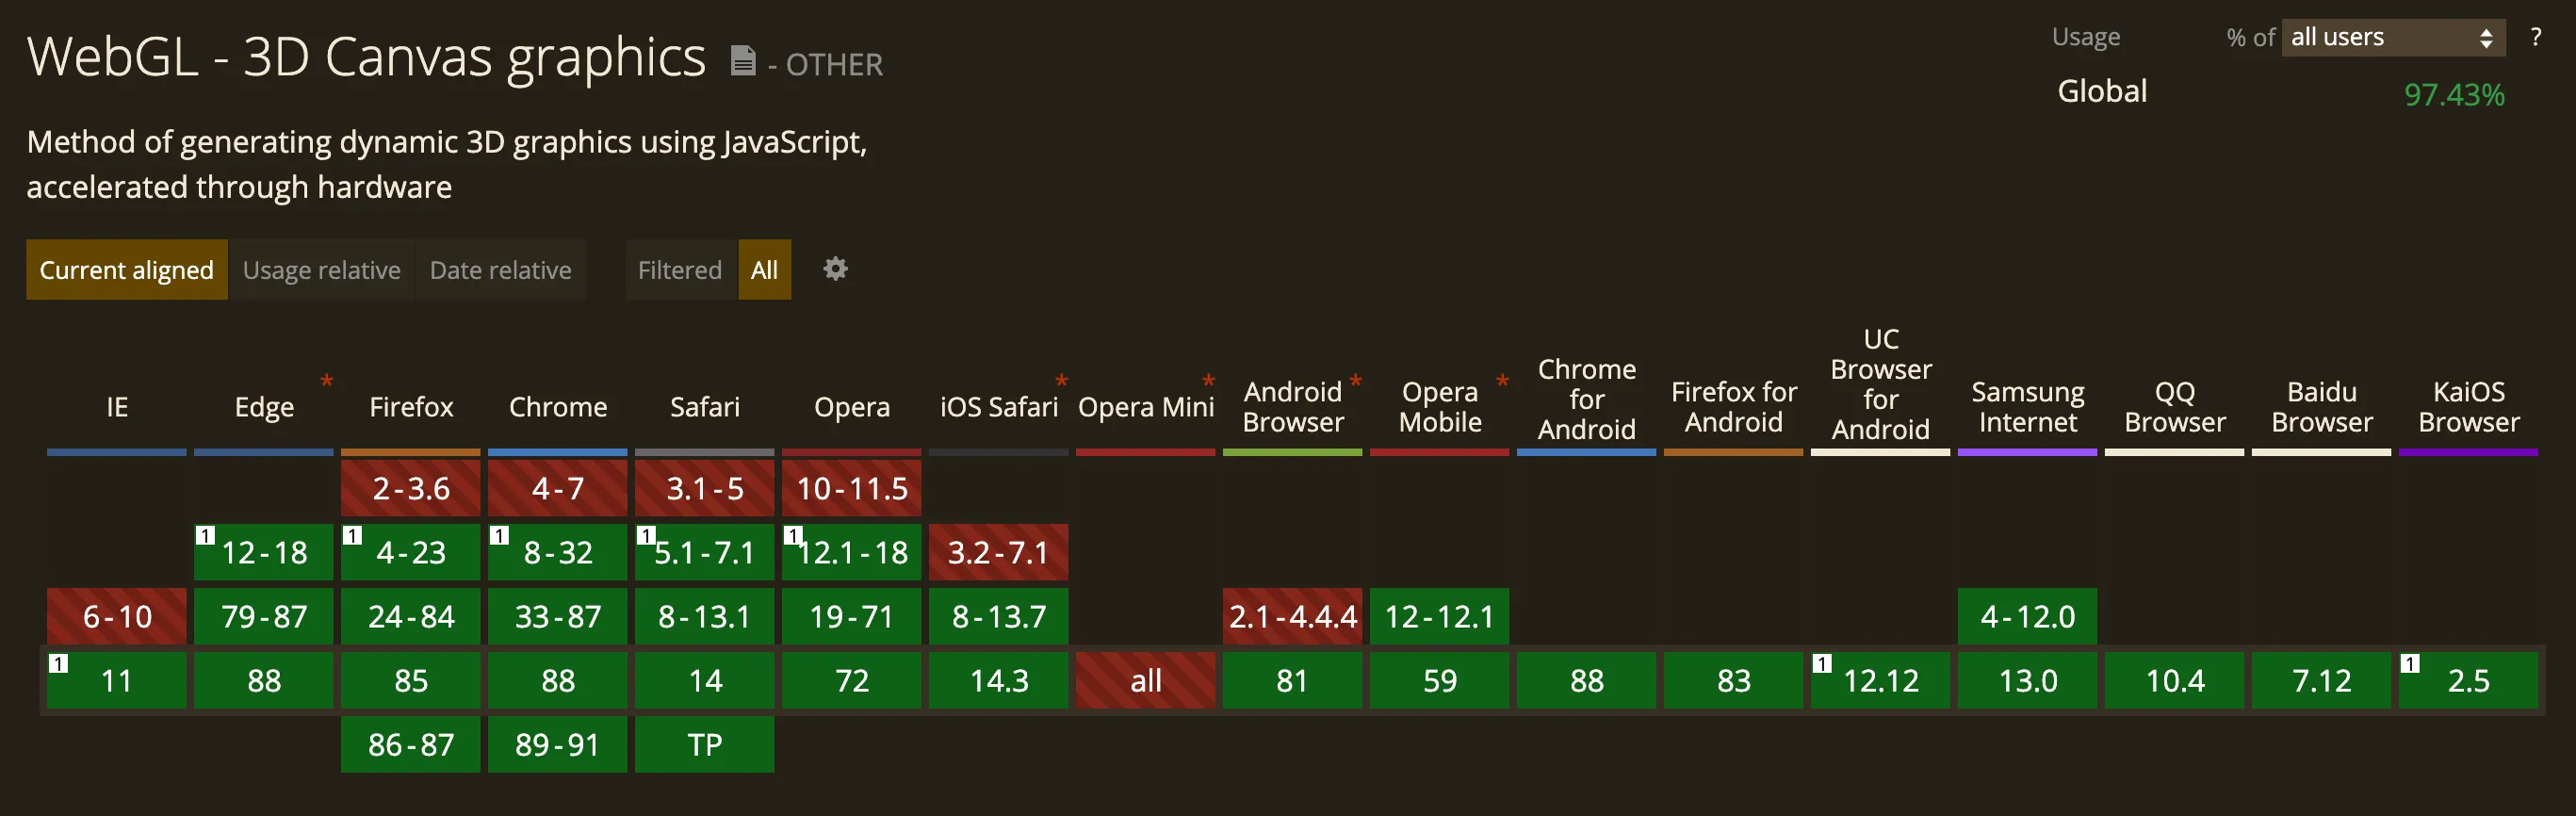
\includegraphics[width=\textwidth]{figures/can-i-use.png}
    \caption[Google Trends data illustrating the ascent of Node.js and React Native.]{\textbf{Google Trends data illustrating the ascent of Node.js (in red) and React Native (in blue) from January 2004 to 2018.} The marked increase aligns with the period when JavaScript began to dominate server-side programming and mobile app development, demonstrating the language’s vice.}
    \label{fig:can-i-use}
  \end{figure}

  Since technologies usually do not vanish overnight, WebGL will for sure stay for many more years. Numerous applications and frameworks rely on WebGL, millions of people use these applications (Similarweb, n.d.), and hundreds of thousands of developers produce new software with WebGL daily, with libraries dependent on WebGL (npm Inc., n.d.). This is understandable because developers can create remarkable things with a low-level graphics API like WebGL. The most famous example is Google Maps — especially Google Earth (Shankland, 2011). Applications like that were unattainable until some years ago, and today, we take it for granted to e.g. interact with 3D content on a website — even on mobile devices!

  WebGL gives developers the JavaScript binding needed to access the computer’s GPU. However, the WebGL API—especially shader programming in the Graphics Library Shader Language (GLSL)—is difficult to use. Therefore, only a few developers grasp and can work with the complexity of WebGL.

  That is why libraries like Three.js, Babylon.js and Playcanvas came into existence. These libraries are basically an abstraction on top of WebGL to render 2D and 3D graphics in the browser via an easy-to-understand JavaScript API. These libraries are widely established and have shown their strength in big production applications (Wappalyzer, n.d.). Nonetheless, WebGL is based on OpenGL ES, a subset of the OpenGL specification designed for browser use, and while OpenGL is a well-established technology, it has some limitations. For instance, it does not support 3D textures, is restricted to triangle meshes, and has various other constraints (The Khronos Group Inc., n.d.). From a high-level view, WebGL is an API built on GPU technology’s understanding from around 15 years ago. Since then, many things have changed. One of the most notable changes is that modern GPUs usually work with shared memory access to perform parallel computing in a more performant fashion than before (Cabello and Wallez, 2019) — and that is where WebGPU comes into play.

  \subsection{Shared Memory}
  \label{subsec:shared-memory}

  To explain it with a beginner’s understanding, shared memory is conceptually a place where each Arithmetic Logic Unit (ALU) can efficiently access the logic of other ALUs instead of calculating it on its own (Wallez, 2020). One can think of shared memory as a hashmap in dynamic programming that can optimise the space-time complexity, e.g. traversing through an input array with constant time operations to access data from the previous iterations instead of calculating them again.

  \begin{figure}[ht]
    \centering
    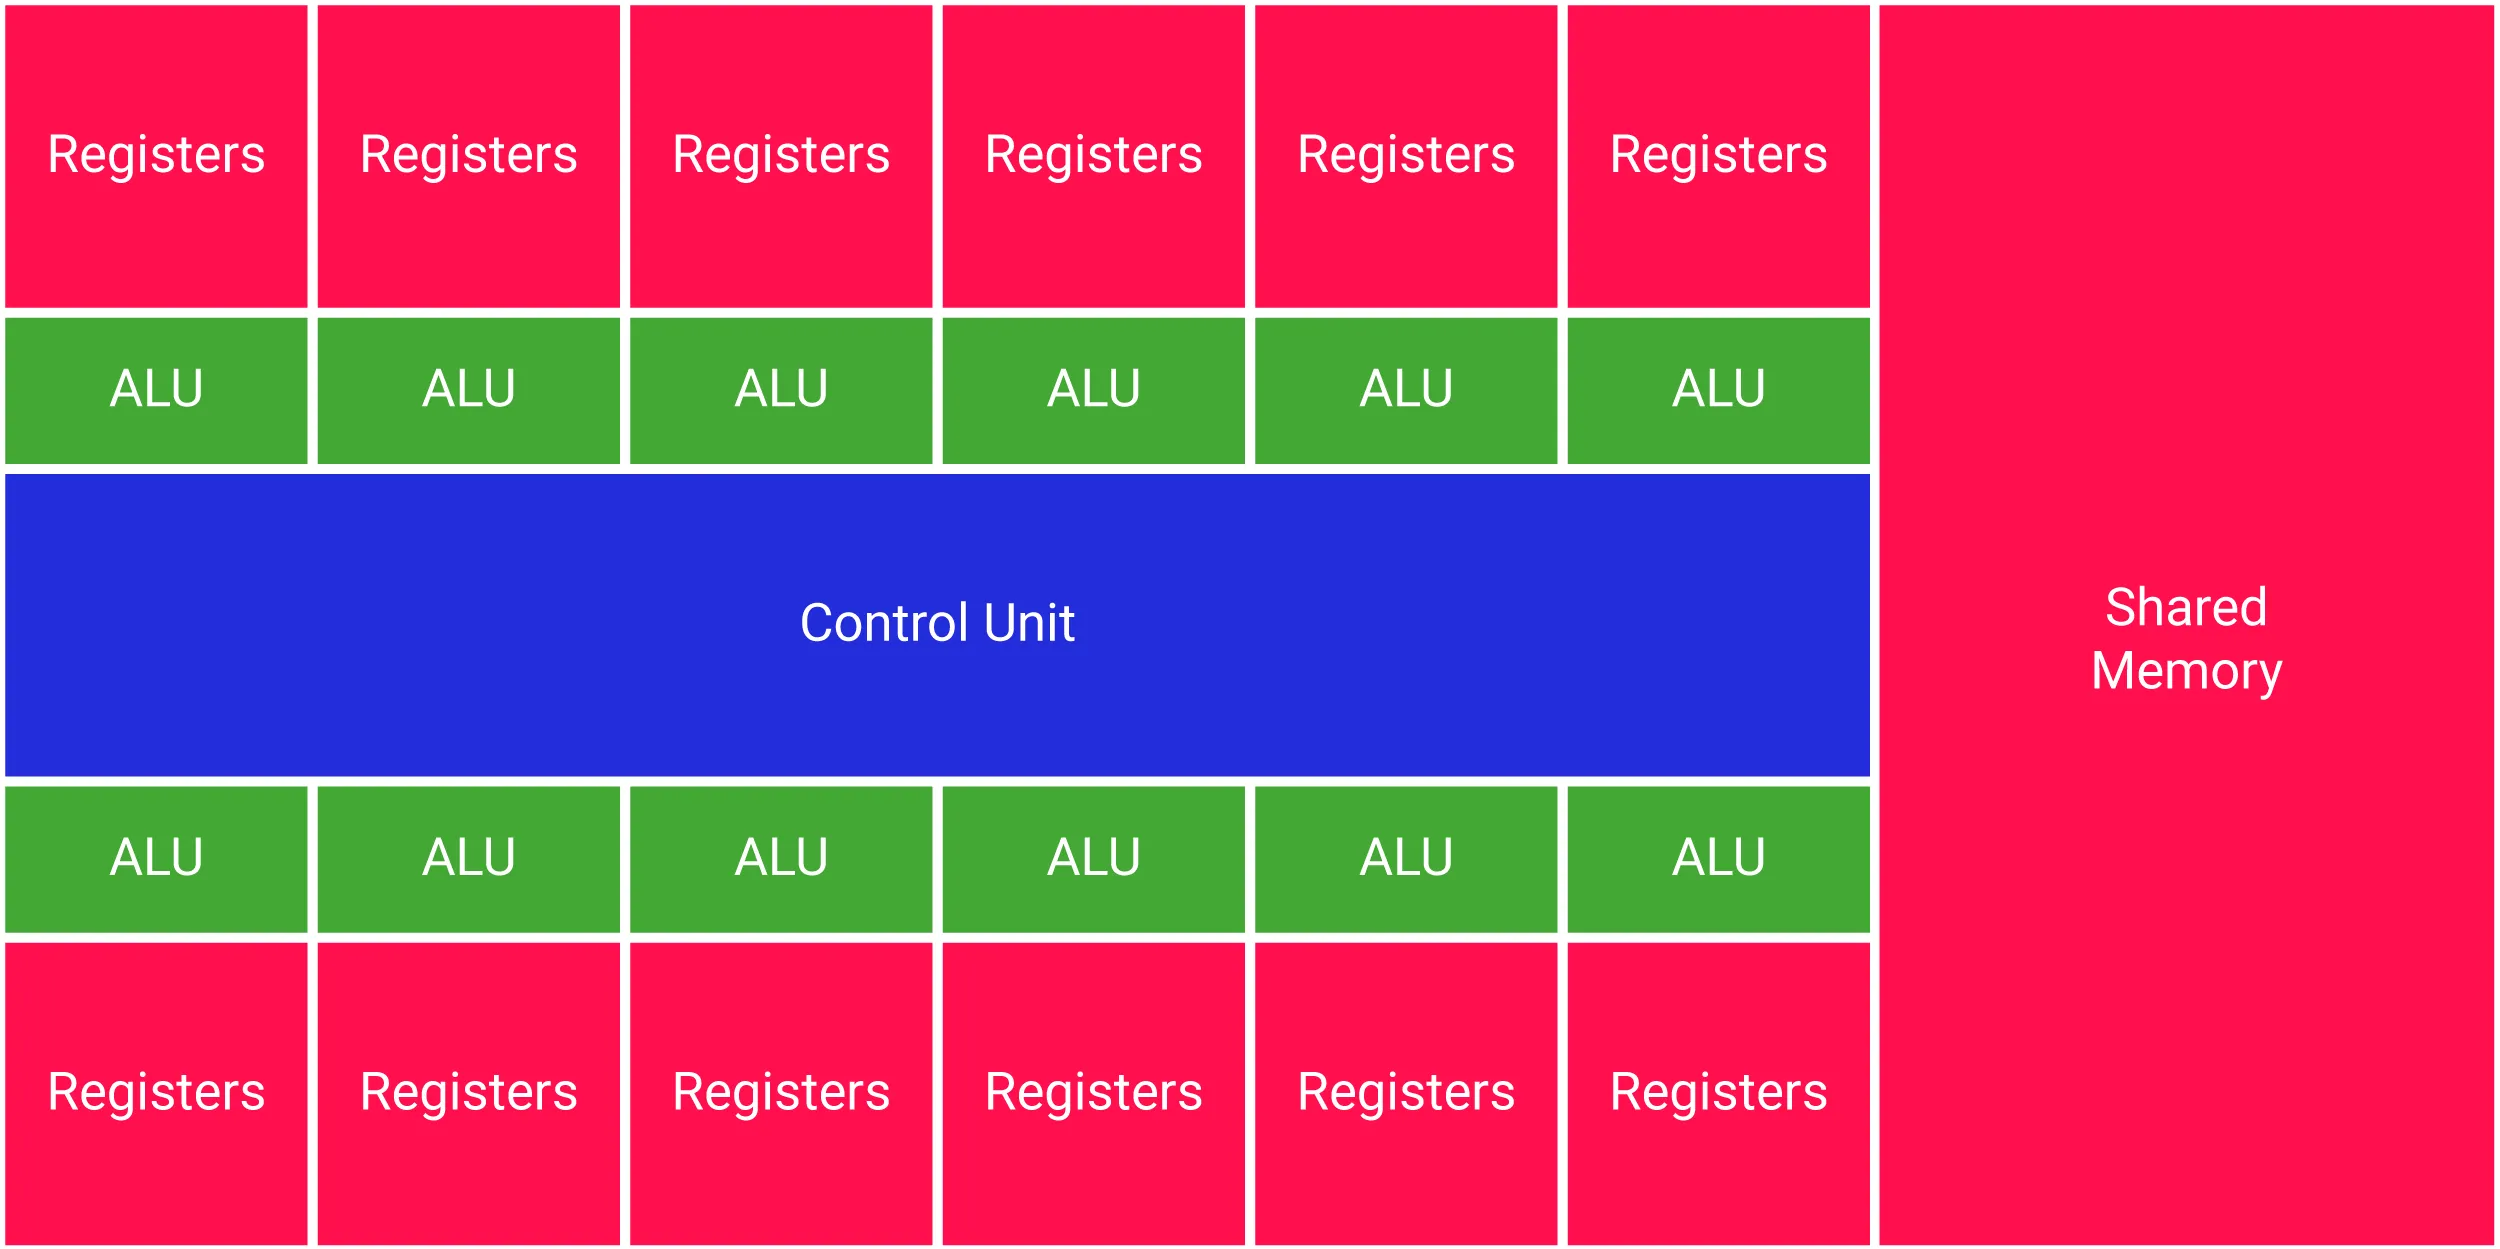
\includegraphics[width=\textwidth]{figures/shared-memory.png}
    \caption[Google Trends data illustrating the ascent of Node.js and React Native.]{\textbf{Google Trends data illustrating the ascent of Node.js (in red) and React Native (in blue) from January 2004 to 2018.} The marked increase aligns with the period when JavaScript began to dominate server-side programming and mobile app development, demonstrating the language’s strengths.}
    \label{fig:shared-memory}
  \end{figure}

  Modern graphics cards APIs such as Vulkan or Metal use concepts like shared memory — and many others — to optimise their performance. One can think comparing OpenGL to, e.g. Vulkan as comparing C to JavaScript: OpenGL — and therefore WebGL too — is slow because the other APIs are closer to the actual hardware and more or less platform-specific optimised as well (Hruska, 2015). OpenGL is not optimised for these new concepts. Many developers switched to Vulkan and Metal due to these new concepts (like shared memory) and the benefits of better performance. However, why can’t we create a new kind of generic OpenGL API that allows talking to all the modern graphics cards? Instead of porting an old native technology to the web, why can’t we create a web API that provides some output that will be understood by the modern APIs (similar to how WebAssembly works with the CPUs (Mozilla Foundation, 2021))? That is precisely what the W3C intends to do with the new WebGPU browser standard.

  \subsection{A Group Effort}
  \label{subsec:a-group-effort}

  WebGPU is a group effort between Apple, Google, Microsoft, and many others, and it is currently being standardised by the W3C to replace WebGL (World Wide Web Consortium, n.d.). Compared to WebGL, WebGPU is not a port of an existing native graphics API to the web. It borrows concepts from, e.g. Vulkan, and aims to provide high performance on modern GPUs thanks to their optimised architecture (Wallez, 2018). It is intended to be able to write WebGPU-specific JavaScript, which all the modern graphics card APIs will understand.

  Additionally, WebGPU is stateless and allows command reuse, meaning that sending instructions to the GPU is less expensive than with WebGL because it creates groups of instructions which will be used in advance (Cabello and Wallez, 2019). It can switch between entire instruction groups at runtime with a single function call (thanks to shared memory). Shortly explained: The current implementation of WebGPU works much faster than WebGL — especially with many 3D object instances in a complex scene.

  \subsection{The Limitation is The User}
  \label{subsec:the-limitation-is-the-user}

  All in all, WebGPU sounds almost too perfect. There is just one thing to consider: We ship the complete source code to the client without knowing their hardware. What if the user visits a super-advanced science visualisation made with modern WebGPU technologies but has only an old onboard graphics card from 5 years ago? Well, it is their fault. It is the same as if a user still uses Internet Explorer in 2021: the typical compatibility misery. However, what if users still need even more elaborate 3D graphics and complex visualisations? What if the requirement exceeds the average consumer hardware? It sounds impossible, but a new type of technology allows developers to tackle this issue.

  \section{Pixel Streaming}
  \label{sec:pixel-streaming}

  Pixel streaming (sometimes called render streaming or remote rendering) allows the audio-visual output of a hosted cloud software to be streamed to the client (Antunes, 2020). The client does not need expensive hardware—only a good internet connection.

  \subsection{How Pixel Streaming Works}
  \label{subsec:how-pixel-streaming-works}

  Basically, pixel streaming is about moving the heavy-lifting logic from the client to the server. It is the concept of developing software on dedicated hardware (with, e.g. dedicated GPUs) and streaming the audio-visual output to the user. As a part of this, client code (like JavaScript) will also be shipped to interact with the server’s software output in real-time (Epic Games Inc., n.d.). This makes pixel streaming, from a developer’s perspective, the less accessible technology compared to WebGL/WebGPU because it relies heavily on expensive hardware.

  \begin{figure}[ht]
    \centering
    \frame{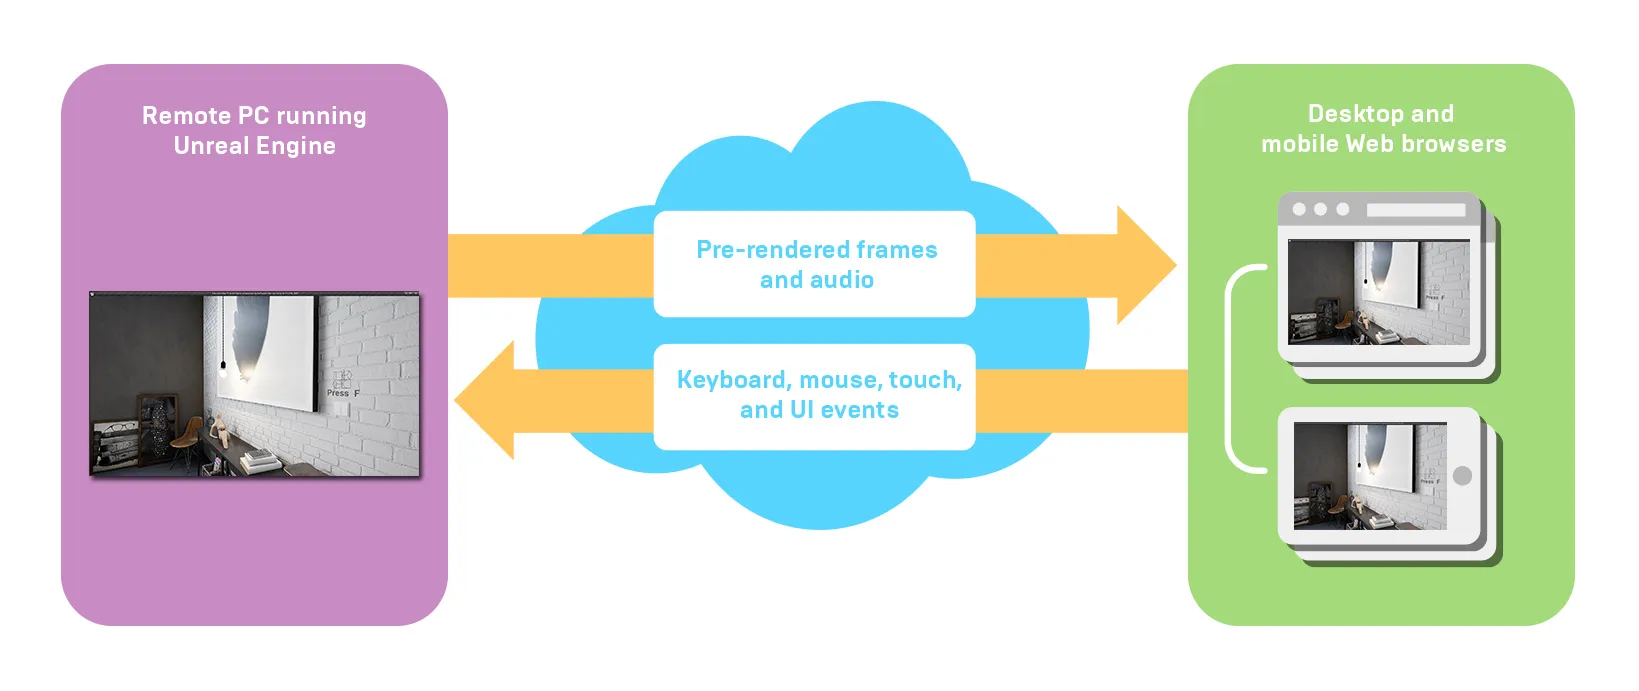
\includegraphics[width=\textwidth]{figures/pixel-streaming-architecture.png}}
    \caption[Google Trends data illustrating the ascent of Node.js and React Native.]{\textbf{Google Trends data illustrating the ascent of Node.js (in red) and React Native (in blue) from January 2004 to 2018.} The marked increase aligns with the period when JavaScript began to dominate server-side programming and mobile app development, demonstrating the language’s strengths.}
    \label{fig:pixel-streaming-architecture}
  \end{figure}

  Nevertheless, with pixel streaming, nearly everything seems possible! Developers can produce cutting-edge software that only runs on high-end graphics cards, which users could never buy or maintain.

  However, that is precisely the problem: scalability. A company/developer needs to gain access to this high-end hardware. Of course, there are Infrastructure as a Service (IaaS) providers like Amazon Web Services (AWS) and Google Cloud Platform (GCP), but there is still a significant limitation: costs. Even with AWS, GCP, and others in the backpack, running software on the required high-end hardware is computationally expensive and consumes much energy (Amazon.com Inc., n.d.). Yes, Google and Co. seem to have endless available computing power, but one would push it to a costly limit with the need for a freely available pixel streaming application.

  \begin{figure}[ht]
    \centering
    
\includegraphics[width=\textwidth]{figures/project-anywhere.jpg}
    \caption[Google Trends data illustrating the ascent of Node.js and React Native.]{\textbf{Google Trends data illustrating the ascent of Node.js (in red) and React Native (in blue) from January 2004 to 2018.} The marked increase aligns with the period when JavaScript began to dominate server-side programming and mobile app development, demonstrating the language’s strengths.}
    \label{fig:project-anywhere}
  \end{figure}

  There are working proof of concepts like the Project Anywhere from NVIDIA, Microsoft and co. with streaming-optimised graphics cards (Woodard and Young, 2020) or (now deprecated) running products like Google Stadia (Patterson, 2020). However, the problem with overcoming the huge price factor is that a company cannot freely give away a pixel streaming application on the web; they would need a payment model for access. Otherwise, the company could ruin itself financially (imagine, e.g. the cost of a DDoS attack on such a free-to-use application).

  \section{Hypothetical App: Virtual Offices}
  \label{sec:hypothetical-app-virtual-offices}

  Now that we know the technologies and some pros and cons let us imagine we want to build a 3D application soon. The application is called Hejm and aims to accommodate people worldwide in a 3D virtual office. No matter what kind of business they run, Hejm provides them with the tools they will need for their remote-only office. Users can enter the office via virtual reality, augmented reality headsets or a standard computer screen.

  \subsection{The Complexity of Pixel Streaming}
  \label{subsec:the-complexity-of-pixel-streaming}

  In a pixel streaming scenario, we would write the Hejm software to run on a cloud GPU instance (e.g. AWS EC2 GPU). We then create a client-side of the software that only provides the interaction JavaScript code to access the server-side logic via a real-time communication protocol. Something to be aware of is the problem that, per accessing user, we would need to fire up an instance with the running software. It is possible to stream the output of one instance to multiple clients (and they can even all interact with it), but that is, yet again, another drawback. In this sense, Multiplayer can — as of today — only be achieved with multiple instances (Epic Games Inc., n.d.), which pushes the costs, too. We can modify our software to optimise it for more than one accessing user per instance. Nonetheless, there is still a vertical limit per GPU.

  Users should also be able to interact with each other in real-time and, therefore, require real-time server communication between instances. The instances also need a single source of truth for updates within the virtual office. There has to be a synchronisation module that updates all the different scenes in the other instances. However, this means that if, e.g. many people move around or do things visible to all the other instances, simple functionalities can already be vast computational tasks and, therefore, costly. On top of this, there should be chat, video, and audio call features within the virtual office application, which are expensive.

  \subsection{A Hybrid Solution}
  \label{subsec:a-hybrid-solution}

  In a perfect hypothetical world, WebGPU would have >95\% browser compatibility, and almost every conventional device would support the new standard, which would be very exciting times for Hejm! Hejm would have different product offerings, ranging from a free version, which runs only in the browser via WebGPU and an enterprise version, which costs around 400\$/month per user. Companies that need the power of pixel streaming — e.g. simulating manufacturing CAD models or the like — would probably also be willing to pay extra for such a remote-first solution (they could at least save on PC hardware and offices for their employees). One could even go further and display certain rooms in the virtual office only via pixel streaming and let the rest run via WebGPU in the browser — therefore being a hybrid solution.

  \section{Conclusion}
  \label{sec:conclusion}

  There is — as with many things — never a simple solution. However, which technology should companies/developers use? One would say that it depends. Creating high-end 3D software that can only run on high-end hardware with limited access and a small user base: develop it with pixel streaming. If the application needs to be served to thousands or millions of users for free but does not require advanced features and visualisations, use WebGPU. If time allows it — and resources for research and development are available — I would encourage companies and developers to create a hybrid to satisfy both worlds’ requirements.

  One can compare it with the discussion between Single-Page Applications (SPAs) and Multi-Page Applications (MPAs): First, the entire page was created on the server and sent as plain HTML/CSS/JS to the client. Then came Angular, React and co., and the UI logic layer shifted to the client; the server was only here to handle and serve the data. However, this solution needed to be more suboptimal: small websites used to send megabytes of JavaScript chunks to display a simple UI (Tsarouva, 2019). This part of the web development industry also goes into a hybrid phase: Server-Side Rendering (SSR) and Incremental Static Generation (ISG). These two different terms deserve an essay of their own. However, They solve the problem by pre-rendering the most critical software parts on the server, and everything that needs to be asynchronous will be put together in the browser (Szczeciński, 2018).

  \section{Outlook}
  \label{sec:outlook}

  The entire front vs. back topic is an ongoing discussion in the web development/software industry. One can assume that there will never be a clear winner. It is exciting to see which of the two opponents in the graphics world will be widely embraced—especially if pixel streaming is a thing to stay and how they want to overcome the high-price drawbacks. Moreover, the hybrid solution might be right, or perhaps an entirely new technology enters the scene.

  % ! ==============================================
  % ! # MARK: References
  % ! ==============================================

  \pagebreak
  \bibliographystyle{../../templates/custom-apa}
  \bibliography{references/bibliography}

\end{sloppypar}
\end{document}
